\documentclass[xcolor=dvipsnames]{beamer}
%\documentclass[handout,xcolor=dvipsnames,pdftex,hyperref={colorlinks=false}]{beamer}

%\usetheme[height=7mm]{Rochester}
\setbeamertemplate{items}[ball]
\setbeamertemplate{blocks}[rounded][shadow=true]
\usepackage{xcolor}
\usepackage{colortbl}
\usepackage{multirow}
\usepackage{amsmath}
\usepackage{amsfonts}
\usepackage{epsfig}
\usepackage{subfigure}
%\usepackage{rotating}
%\usepackage{theorem}

%\usepackage{tikz}
%\usetikzlibrary{arrows,positioning,shapes}

\usepackage{tikz}
\usetikzlibrary{shapes,decorations,arrows,calc,arrows.meta,fit,positioning}
\tikzset{
	-latex,auto,node distance = 2cm and 2cm,
	thick,
	state/.style ={ellipse, draw, minimum width = 2cm},
	el/.style = {inner sep=3pt, align=left, sloped},
	point/.style = {circle, draw=black, inner sep=0.04cm,
     fill=black,node contents={}},
    bidirected/.style={Latex-Latex,dashed},
}



\usepackage{times}
\usepackage[T1]{fontenc}
\usepackage{inconsolata}
\usepackage{fancyvrb}

% == theme & colors
\usetheme{Warsaw}
\usepackage{helvet}
\definecolor{someblue}{rgb}{0,.1,0.8}

\title{Stat 256: Causality}
\subtitle[ ]{Instrumental Variables}
\author{Chad Hazlett}
\date{Spring 2026}
\institute[UCLA]{UCLA\\[1ex]
  \texttt{chazlett@ucla.edu}}
%\date{}

\definecolor{dgreen}{rgb}{0,.6,0.8}
\newtheorem{assumption}{Assumption}
\newtheorem{iass}{Identification Assumption}
\newtheorem{ires}{Identification Result}
\newtheorem{estm}{Estimand}
\newtheorem{esti}{Estimator}
\newtheorem{question}{Question}
\newtheorem{answer}{Answer}
\newtheorem{proposition}{Proposition}
\newcommand{\bs}{\boldsymbol}
\newcommand{\mb}{\mathbf}
\newcommand{\real}{\mathbb{R}}
\renewcommand{\u}{\ensuremath{\mb{u}}}
\renewcommand{\v}{\ensuremath{\mb{v}}}
\newcommand{\U}{\ensuremath{\mb{U}}}
\newcommand{\Z}{\ensuremath{\mb{Z}}}
\newcommand{\PP}{\ensuremath{\mb{P}}}
\newcommand{\M}{\ensuremath{\mb{M}}}
\newcommand{\X}{\ensuremath{\mb{X}}}
\newcommand{\x}{\ensuremath{\mb{x}}}
\newcommand{\Y}{\ensuremath{\mb{Y}}}
\newcommand{\D}{\ensuremath{\mb{D}}}
\newcommand{\y}{\ensuremath{\mb{y}}}
\renewcommand{\b}{\ensuremath{\bs{\beta}}}
\newcommand{\e}{\ensuremath{\bs{\epsilon}}}
\newcommand{\bhat}{\ensuremath{\hat{\bs{\beta}}}}
\newcommand{\XX}{\ensuremath{\X'\X}}
\newcommand{\XXinv}{\ensuremath{\left(\XX\right)^{-1}}}
\newcommand{\hatsig}{\ensuremath{\hat{\sigma}^2}}
\newcommand{\sig}{\ensuremath{\sigma^2}}
\newcommand{\hatmat}{\ensuremath{\X \XXinv \X'}}
\newcommand{\ehat}{\ensuremath{\hat{\e}}}
\newcommand{\tr}{\text{tr}}
\newcommand{\Sig}{\ensuremath{\bs{\Sigma}}}
\newcommand{\SigInv}{\ensuremath{\bs{\Sigma^{-1}}}}
\newcommand{\W}{\ensuremath{\mb{W}}}
\newcommand{\E}{\mathbb{E}}
\newcommand{\V}{\mathbb{V}}
\newcommand{\inprob}{\stackrel{p}{\rightarrow}}


\newcommand{\indep}{{\bot\negthickspace\negthickspace\bot}}

% --- Additions for IV-OVB sensitivity coda (added 2026-04-29) ---
\usepackage{appendixnumberbeamer}
\usepackage{booktabs}
\usepackage{bm}
\newcommand{\R}{{\bm R}}
\DeclareMathOperator*{\plim}{plim}
\DeclareMathOperator{\rank}{rank}
\DeclareMathOperator{\sgn}{sgn}
\DeclareMathOperator{\var}{var}
\DeclareMathOperator{\cov}{cov}
\DeclareMathOperator{\cor}{cor}
\DeclareMathOperator{\sd}{sd}
\DeclareMathOperator{\se}{se}
\DeclareMathOperator{\df}{df}
\DeclareMathOperator{\rv}{RV}
\DeclareMathOperator{\xrv}{XRV}
\DeclareMathOperator{\iv}{IV}
\DeclareMathOperator{\rf}{RF}
\DeclareMathOperator{\fs}{FS}
\DeclareMathOperator{\ar}{AR}
\DeclareMathOperator{\bias}{bias}
\DeclareMathOperator{\BF}{BF}
\DeclareMathOperator{\SeF}{SeF}
% --- end additions ---

\useoutertheme{infolines}
\begin{document}

\subject{Talks}
\AtBeginSection[]
{
  \begin{frame}<beamer>
    \frametitle{Outline}
    \tableofcontents[currentsection]
  \end{frame}
}

\AtBeginSubsection[]
{
  \begin{frame}<beamer>
    \frametitle{Outline}
    \tableofcontents[currentsection,currentsubsection]
  \end{frame}
}

\begin{frame}
  \titlepage
\end{frame}

\section{IV setup}\label{iv-setup}

\begin{frame}{Where are we? Where are we going?}

\begin{itemize}[<+->]
\small
\item
  We know now what to do when we can argue for backdoor/CI.
  \medskip
\item
  And we know we can use do-calc to find any other adjustment that, given a non-parametric DAG \textcolor{red}{and no other assumptions}, can ID an effect (including front-door, napkin, and any others if one exists.
    \medskip
\item
Next we consider other options, all of which require some assumption not represented non-parametrically by an SCM/DAG. 
\medskip
\item
First up: \textcolor{Blue}{Instrumental variables} (IV): ``what if you can find an\textcolor{Blue}{exogenous sources of variation} that drives the
  treatment?''
\end{itemize}
\end{frame}

%================================================================
% Encouragement-design intuition (lifted from PS200C 07-iv/IV.tex,
% pizza -> fitness-program voucher; outcome is BP)
%================================================================
\begin{frame}{The intuition: a randomized encouragement}
\onslide<1-> Suppose we can't randomize \textit{joining a fitness program} (we can't force people to exercise, and we shouldn't forbid them either), but we \textit{can} randomize a \textit{free voucher} for a 12-week program.\\
\bigskip
\onslide<2-> Half the sample gets a voucher; we observe who actually enrolls, then measure blood pressure (BP).\\
\bigskip
\onslide<3-> \textcolor{Blue}{Good news:} we have an experiment with respect to the voucher.
\begin{itemize}
\item<4-> $\E[\text{BP} \mid \text{voucher}] - \E[\text{BP} \mid \text{no voucher}]$ is identified.\\
This is the \textcolor{Blue}{intent-to-treat (ITT)} or \textcolor{Blue}{reduced form} effect of the voucher.
\item<5-> \textcolor{Red}{But it isn't the effect of the program.} How do we get back to that?
\end{itemize}
\end{frame}

\begin{frame}{Backing it out: four kinds of people}
\onslide<1-> Imagine four groups defined by how they respond to the encouragement:
\small
\begin{itemize}
\item<2-> \textit{Never-takers}: don't enroll either way. \textcolor{Blue}{Voucher has no effect on their enrollment $\Rightarrow$ no effect on their BP.}
\smallskip
\item<3-> \textit{Always-takers}: enroll either way. \textcolor{Blue}{Same: voucher doesn't change anything for them.}
\smallskip
\item<4-> \textit{Compliers}: enroll \textit{iff} they get the voucher. \textcolor{Blue}{For them, voucher means program, no voucher means no program: effect of voucher (ITT) is effect of program.}
\smallskip
\item<5-> \textit{Defiers}: enroll \textit{iff} they don't get the voucher. \textcolor{Red}{We assume away.}
\end{itemize}
\bigskip
\onslide<6-> \normalsize \textcolor{Blue}{Punchline:} the ITT over everyone will be an average over these and so will be a \textit{watered-down} version of the program effect. Specifically,
\end{frame}

\begin{frame}{Backing it out: the algebra}
\small
\onslide<1-> Averaging the ITT over the four types:\\
\footnotesize
\begin{align*}
\text{ITT} \;=\; & \underbrace{(\text{ITT}\mid \text{never-taker})}_{=0}\cdot \Pr(\text{never-taker}) \\
&+\; \underbrace{(\text{ITT}\mid \text{always-taker})}_{=0}\cdot \Pr(\text{always-taker}) \\
&+\; \textcolor{Blue}{(\text{ITT}\mid \text{complier})\cdot \Pr(\text{complier})} \\
&+\; \underbrace{(\text{ITT}\mid \text{defier})}_{=0,\;\text{by assumption}}\cdot \Pr(\text{defier}) \\[2pt]
\Rightarrow\quad \text{ITT}\mid\text{complier} \;=\;& \frac{\text{ITT}}{\Pr(\text{complier})}
\end{align*}
\medskip
\onslide<2-> \normalsize \textcolor{Blue}{So we can recover an ITT-for-compliers.} \\
\medskip
\onslide<3-> And for compliers, the ITT is the ATE.
\end{frame}

\begin{frame}{From ITT-on-compliers to LATE}
\small
\onslide<1-> One more thing you need to know: $\Pr(\text{complier})$ is the ``first stage'' effect:\\

\bigskip

$\Pr(\text{complier}) = \E[D_1 - D_0] = \E[D|Z=1]-\E[D|Z=0]$ (by ignorability of $Z$), which equals the proportion of compliers (if no defiers).

\bigskip

\onslide<4-> \small Putting it together: We call the ATE among the compliers the ``local average treatment effect'' (LATE):

\begin{center}
\textcolor{Blue}{$\displaystyle \text{LATE} \;=\; \frac{\text{ITT}}{\text{Pr(complier)}}\; = \; \frac{\E[Y\mid Z=1]-\E[Y\mid Z=0]}{\E[D\mid Z=1]-\E[D\mid Z=0]}$}
\end{center}
\end{frame}

%================================================================
% Now back to the formal IV setup
%================================================================

\begin{frame}{Basic IV setup with DAGs}

\begin{center}
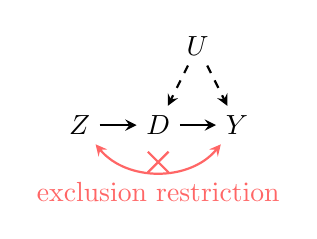
\begin{tikzpicture}
    \node (z1) at (-1,0) {$Z$};
    \node (a1) at (0,0) {$D$};
    \node (l1) at (0.5, 1)
    {$U$};
    \node (y) at
    (1,0) {$Y$};
    \draw[->, >=stealth, thick, dashed] (l1) -- (a1);
    \draw[->, >=stealth, thick, dashed] (l1) --  (y);
    \draw[->, >=stealth, thick] (a1) -- (y);
    \draw[->, >=stealth, thick] (z1) -- (a1);
    \onslide<2->{\draw[<->, >=stealth, red!60, thick] (z1)  to[bend right = 50] node[cross out, -, draw, red!60, thick, midway] {\vspace{3em}} node[red!60, midway, below] {exclusion restriction}(y);}
\end{tikzpicture}
\end{center}

\pause

\begin{itemize}[<+->]
\small
\item
  \(Z\) is the instrument, \(D\) is the treatment, and \(U\) is the
  unmeasured confounder
\item
  Absence of $Z-Y$ arc, however directed, is known by two assumptions:
  \begin{itemize}[<+->]
  \item
    no common causes of instrument and the outcome (\textcolor{Blue}{exogeneity})
  \item
    no direct or indirect effect of the instrument on the outcome except through treatment (\textcolor{Blue}{exclusion})
  \end{itemize}
\item
  First-stage relationship: \(Z\) affects \(D\)  (\textcolor{Blue}{relevance})
  \item Actually Z-D confounding is workable, but ruled out in one popular framework we will look at. 
  \end{itemize}
\end{frame}

%\begin{frame}
%\begin{figure}[t]
%    \begin{tikzpicture}[node distance = 2cm]
%        \node (z) [label = left:$Z$, point];
%        \node (d) [label = above left:$D$, point,  right of = z];
%        \node[below of = d, node distance = 1.45cm, color = transparent] (w) {};
%        \node (y) [label = right:$Y$, point,  right of = d];
%        \node (x) [label = above:$X$, point,  above of = d, node distance = 1cm];
%        \path (z) edge  (d);
%        \path (d) edge  (y);
%        \path (x) edge  (z);
%        \path (x) edge  (d);
%        \path (x) edge  (y);
%        \path[dashed, transparent] (w) edge  (z);
%        \path[dashed, transparent] (w) edge  (d);
%        \path[dashed, transparent] (w) edge  (y);
%       % \path[dashed, red] (w) edge  (x);
%        \path[latex-latex,dashed] (d) edge[bend left= 20] (y);
%    \end{tikzpicture}
%    \caption{}
%    \label{fig:iv1}
%% \begin{subfigure}[b]{0.33\linewidth}
%% \centering
%    \begin{tikzpicture}[node distance = 2cm]
%        \node (z) [label = left:$Z$, point];
%        \node (d) [label = above left:$D$, point,  right of = z];
%        \node (w) [label = below:$W$, point,  below of = d, node distance = 1cm];
%        \node (y) [label = right:$Y$, point,  right of = d];
%        \node (x) [label = above:$X$, point,  above of = d, node distance = 1cm];
%        \path (z) edge  (d);
%        \path (d) edge  (y);
%        \path (x) edge  (z);
%        \path (x) edge  (d);
%        \path (x) edge  (y);
%        \path[dashed, red] (w) edge  (z);
%        \path[dashed, red] (w) edge  (d);
%        \path[dashed, red] (w) edge  (y);
%        % \path[dashed, red] (w) edge  (x);
%        \path[latex-latex,dashed] (d) edge[bend left= 20] (y);
%    \end{tikzpicture}
%%    \caption{}
%%    \label{fig:iv2}
%% \end{subfigure}%
%%  \begin{subfigure}[b]{0.33\linewidth}
%% \centering
%    \begin{tikzpicture}[node distance = 2cm]
%        \node (z) [label = left:$Z$, point];
%        \node (d) [label = above left:$D$, point,  right of = z];
%        \node (w) [label = below:$W$, point,  below of = d, node distance = 1cm];
%        \node (y) [label = right:$Y$, point,  right of = d];
%        \node (x) [label = above:$X$, point,  above of = d, node distance = 1cm];
%        \path (z) edge  (d);
%        \path (d) edge  (y);
%        \path (x) edge  (z);
%        \path (x) edge  (d);
%        \path (x) edge  (y);
%        \path[dashed, red] (z) edge  (w);
%        \path[dashed, red] (w) edge  (d);
%        \path[dashed, red] (w) edge  (y);
%        % \path[dashed, red] (w) edge  (x);
%        \path[latex-latex,dashed] (d) edge[bend left= 20] (y);
%    \end{tikzpicture}
% %   \caption{}
% %   \label{fig:iv3}
%% \end{subfigure}
%% \caption{Causal diagrams illustrating traditional IV assumptions. In Figure~\ref{fig:iv1}, $X$ is sufficient for rendering $Z$ a valid instrumental variable. In Figures~\ref{fig:iv2}~and~\ref{fig:iv3}, however, $W$ is also needed to render $Z$ a valid IV, either because it confounds the instrument-outcome relatonship (Fig.~\ref{fig:iv2}) or because it is a side-effect of the instrument affecting the outcome other than through its effect of on the treatment (Fig.~\ref{fig:iv3}). In practice, all these violations will be happening simulatanously. Graphically, conditional on a set of covariates $\{X, W\}$,  $Z$ is a valid instrumental variable for the causal effect of  a treatment $D$ on an outcome $Y$, if the set $\{X, W\}$ blocks all paths from $Z$ to $Y$ on the graph where the edge $D\rightarrow Y$ is removed~\citep{brito2002generalized}.}
%%\label{fig:ovb4iv-examples}
%\end{figure}
%\end{frame}


\begin{frame}{Basic IV setup with DAGs}

\begin{center}
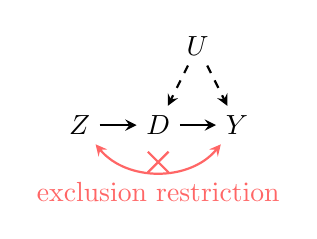
\begin{tikzpicture}
    \node (z1) at (-1,0) {$Z$};
    \node (a1) at (0,0) {$D$};
    \node (l1) at (0.5, 1)
    {$U$};
    \node (y) at
    (1,0) {$Y$};
    \draw[->, >=stealth, thick, dashed] (l1) -- (a1);
    \draw[->, >=stealth, thick, dashed] (l1) --  (y);
    \draw[->, >=stealth, thick] (a1) -- (y);
    \draw[->, >=stealth, thick] (z1) -- (a1);
    \onslide<2->{\draw[<->, >=stealth, red!60, thick] (z1)  to[bend right = 50] node[cross out, -, draw, red!60, thick, midway] {\vspace{3em}} node[red!60, midway, below] {exclusion restriction}(y);}
\end{tikzpicture}
\end{center}

\onslide<1-> The IV-DAG irony:
\begin{itemize}
\item<2-> DAGs are great to convey the IV idea; even anti-DAGs probably draw one in the air when they talk about IV.

\item<3-> But, DAGs+do-calc won't tell you that IV identifies a causal effect:
\begin{itemize} 
\item<4-> Identification depends on a ``monotonicity'' assumption ($Z$ only affects $D$ in one direction)
%\item<5-> Though analysis of the DAG still generates insights regarding what to expect if the DGP follows the IV setup above, including some interesting bounds (Pearl, 1995)
%\item<6-> We'll also talk about sensitivity analyses regarding those violations
\end{itemize}
\end{itemize}
\end{frame}

%\begin{frame}{An IV is only as good as its assumptions}
%
%\begin{center}
%\begin{tikzpicture}
%    \node (z1) at (-1,0) {$Z$};
%    \node (a1) at (0,0) {$D$};
%    \node (l1) at (0.5, 1)
%    {$U$};
%    \node (y) at
%    (1,0) {$Y$};
%    \draw[->, >=stealth, thick, dashed] (l1) -- (a1);
%    \draw[->, >=stealth, thick, dashed] (l1) --  (y);
%    \draw[->, >=stealth, thick] (a1) -- (y);
%    \draw[->, >=stealth, thick] (z1) -- (a1);
%    \draw[<->, >=stealth, red!60, thick] (z1)  to[bend right = 50] node[cross out, -, draw, red!60, thick, midway] {\vspace{3em}} node[red!60, midway, below] {exclusion restriction}(y);
%\end{tikzpicture}
%\end{center}
%\small
%\begin{itemize}[<+->]
%\item
%  Finding a believable instrument is difficult and some
%  people skeptical of any IV setup except those arising from randomizing $Z$
%  \item Indeed, $Z$ may be treatment \textit{assignment}, but due to non-compliance, it is not actual treatment. This is a vital use-case for instruments. 
%%\item
% % When effects vary, the IV approach estimates a ``local'' ATE that is
%  % local to this particular instrument.
%\end{itemize}
%\end{frame}

\begin{frame}{IVs in empirical work}
\small
\onslide<1-> Uses of IV with randomization:
\footnotesize
\begin{itemize}[<+->]
\item Killer application: RCTs with non-compliance.  ITT is unbiased, but IV is the undiluted effect of treatment (in the compliers)
\item Randomized encouragement designs are also great way to get an RCT from a non-randomizable treatment. 
\end{itemize}
\small
\onslide<2-> Then there are observational studies that attempt to ``find an instrument''. More challenging. To give you a flavor:\\
\footnotesize
\begin{itemize}[<+->]
\item
  Angrist (1990): Draft lottery as an IV for military service (income as
  outcome)
\item
  Acemoglu et al (2001): settler mortality as an IV for institutional
  quality (GDP/capita as outcome)
\item
  Levitt (1997): being an election year as IV for police force size
  (crime as outcome)
\item
  Kern \& Hainmueller (2009): having West German TV reception in East
  Berlin as an instrument for West German TV watching (outcome is
  support for the East German regime)
%\item
%  Nunn \& Wantchekon (2011): historical distance of ethnic group to 
%  coast as instrument for exposure to slave raids  (outcome are trust attitudes today)
\item
  Acharya, Blackwell, Sen (2015): cotton suitability as IV for
  proportion of population in slavery in 1860 (outcome is white attitudes today)
\end{itemize}

\end{frame}

\begin{frame}{IV then and now}
\begin{itemize}
\item<2-> IV was originally framed as a system of structural equations with constant treatment effects, estimated by 2SLS. Useful intuition, but ties identification to a strong constancy assumption.
\medskip
\item<3-> We'll work mostly in the modern \emph{potential outcomes} language --- LATE, compliers, monotonicity --- which makes assumptions and target estimand transparent under heterogeneity.
\medskip
\item<4-> The SEM/2SLS treatment is in the appendix for reference (and because you'll see it everywhere in applied work).
\end{itemize}
\end{frame}


\section{The new way: with potential outcomes and heterogeneity}

\begin{frame}
  \frametitle{POM for Instrumental Variables}
\onslide<1-> \begin{definition}[Instrument]
$Z_i$: Binary instrument for {\em unit} $i$.
 \[
 Z_i = \left\{
 \begin{array}{ll}
  1 & \mbox{if unit $i$ ``encouraged'' to receive treatment}\\
  0 & \mbox{if unit $i$ ``encouraged'' to receive control}
 \end{array}
 \right.
 \]
\end{definition}

\onslide<2-> \begin{definition}[Potential Treatments]
 $D_{zi}$ indicates \emph{potential} treatment status given $Z_i=z$
%\begin{itemize}
%\item e.g. if $D_{1i}=1$, $i$ was encouraged to take treatment and does
%\end{itemize}
\end{definition}

\onslide<3-> \begin{assumption}[Consistency  of potential treatments]
Observed treatments are realized as
\[
D_i = Z_i \cdot D_{1i}+(1-Z_i)\cdot D_{0i} \,\, \mbox{so}\,\,
D_i = \left\{
 \begin{array}{ll}
  D_{1i} & \mbox{if $Z_i=1$}\\
  D_{0i} & \mbox{if $Z_i=0$}
 \end{array}
 \right.
\]
\end{assumption}
\end{frame}


\begin{frame}
\frametitle{Potential Outcome Model for Instrumental Variables}
Following Angrist, Imbens, and Rubin (1996), we can define:\bigskip
\begin{Definition}
\begin{itemize}
 \item {\em Compliers}: $D_{1i}>D_{0i}$ ($D_{0i}=0$ and $D_{1i}=1$).
 \item {\em Always-takers}: $D_{1i}=D_{0i}=1$.
 \item {\em Never-takers}: $D_{1i}=D_{0i}=0$.
 \item {\em Defiers}: $D_{1i}<D_{0i}$ ($D_{0i}=1$ and $D_{1i}=0$).
\end{itemize}
\end{Definition}
\small
\onslide<2->  Only  $(D_{0i}$ or $D_{1i})$ is observed, not both, so we cannot identify which group an individual belongs to.
\begin{itemize}
\item<3-> Though, further assumptions often help, e.g. no defiers, and sometimes no always-takers. 
\end{itemize}
\end{frame}

%\begin{frame}
%  \frametitle{\small Who are the Compliers? Is exclusion restriction reasonable?}
%  \begin{center}
%  \includegraphics[height=2.55in,keepaspectratio=1]{IVexamples.pdf}\
%  \end{center}
%\end{frame}

\begin{frame}
  \frametitle{Potential Outcome Model for Instrumental Variables}
  \small
\begin{definition}[Potential Outcomes]
Given the binary instrument $Z_i \in \{1,0\}$ and the binary treatment $D_i \in \{1,0\}$ every unit now has four potential outcomes $Y_i(D,Z)$:
$$Y_i(D_i=1,Z_i=1);\; Y_i(D_i=1,Z_i=0);\; Y_i(D_i=0,Z_i=1);\; Y(D_i=0,Z_i=0)$$
%%e.g. the causal effect of the treatment given the unit's realized encouragement status is given by $Y(D=1,Z_i)-Y(D=0,Z_i)$.
\end{definition}

\bigskip
\begin{itemize}
\item<2-> Under exclusion restriction, we will have  $Y_i(d,z=0)=Y(d,z=1) = Y_i(d)$ 
%\item<5-> Exclusion also baked in under assumption $\{ Y_{0i},Y_{1i} \} \indep Z_i$. How so?
\end{itemize}
%  $\rightarrow$ we can index potential outcomes solely by treatment status: ($Y_{1i}$,$Y_{0i}$
%\begin{assumption}[1. Ignorability of the Instrument]
%\[ \{Y_{0i},Y_{1i}, D_{0i},D_{1i}\} \indep Z_i \]
%\vspace{-.2in}
%\small
%\begin{enumerate}
%  \item Independence: Since $Z_i$ independent of all potential outcomes and potential treatments $(Y_i(d,z), D_{1i},D_{0i})\indep Z_i$ for all $d,Z$. Implies identifiability of effects of $Z_i$ on $Y_i$ and $Z_i$ on $D_i$.
%  \item Exclusion implied by $(Y_{0i},Y_{1i}) \indep Z_i$.\\
%   \smallskip \footnotesize Note, $Y_i(d,0)=Y(d,1)$ for all $d$ 
%  $\rightarrow$ we can index potential outcomes solely by treatment status: ($Y_{1i}$,$Y_{0i}$)
%\end{enumerate}
%\end{assumption}
%
\end{frame}


\begin{frame}
  \frametitle{Potential Outcome Model for Instrumental Variables}
\begin{estm}[LATE]
\small
$$\alpha_{LATE}=\E[Y_{1i}-Y_{0i}|D_{1i}>D_{0i}]$$ is the Local Average Treatment Effect among compliers.\\ \smallskip \footnotesize NB: this estimand varies with the particular instrument $Z$. 
\end{estm}
\normalsize
\onslide<2-> Some special cases: 
\footnotesize
\begin{itemize}
\item<2-> When the treatment intake, $D_i$, is itself randomized, \pause then $Z_i=D_i$ and every individual is a complier
\item<3-> If one-sided noncompliance s.t. $D_{0i}=0$: \pause
\end{itemize}
\begin{equation*}
\begin{split}
\E[Y_{1i}|D_{1i}>D_{0i}]&=\E[Y_{1i}|Z_i=1,D_{1i}=1]=\E[Y_{1i}|D_i=1]\\ 
&\mbox{And}\\
\E[Y_{0i}|D_{1i}>D_{0i}]&=\E[Y_{0i}|D_i=1]
\end{split}
\end{equation*}
Thus, 

$$\alpha_{LATE}=\E[Y_{1i}-Y_{0i}|D_{1i}>D_{0i}]=\E[Y_{1i}-Y_{0i}|D_i=1]=\alpha_{ATT}$$
\end{frame}

\subsection{Identification}

\begin{frame}
  \frametitle{Identification of the LATE under IV}
\begin{iass}
\small
\begin{enumerate}
  \item Ignorability of the Instrument: $(Y_{0i},Y_{1i}, D_{0i},D_{1i}) \indep Z_i$
  \item First Stage:  $P(D_{1i}=1) \neq P(D_{0i}=1)$
  \item Monotonicity: $D_{1i} \geq D_{0i}$ for all $i$ (no defiers)
  \end{enumerate}
\end{iass}\vspace{-.2in}
\bigskip
\onslide<2->
\begin{ires}
\footnotesize
\begin{align*}
 \E[Y_1-Y_0|D_1>D_0] &= \frac{\E[Y|Z=1]-\E[Y|Z=0]}{\E[D|Z=1]-\E[D|Z=0]} \\
   &= \frac{\mbox{Intent to Treat Effect of $Z$ on $Y$}}{\mbox{First Stage Effect of $Z$ on $D$}} \\
   &= \frac{\mbox{Intent to Treat Effect}}{\mbox{Proportion of Compliers}}
\end{align*}
\end{ires}
\end{frame}


\begin{frame}
  \frametitle{Identification of the LATE under IV}
\begin{iass}
\small
\begin{enumerate}
  \item Ignorability of the Instrument: $(Y_{0i},Y_{1i}, D_{0i},D_{1i}) \indep Z_i$
  \item First Stage:  $P(D_{1i}=1) \neq P(D_{0i}=1)$
  \item Monotonicity: $D_{1i} \geq D_{0i}$ for all $i$ (no defiers)
  \end{enumerate}
\end{iass}\vspace{-.2in}
\bigskip
\onslide<2->
\begin{ires}[Intuition]
\footnotesize
Intuition:
\begin{itemize}
\item<3-> Effect of $Z$ on $Y$ is identified (ITT)
\item<4-> Effect of $Z$ on $D$ is identified and is the $Pr(complier)$
\item<5-> All of the effect of $Z$ on $Y$ is through compliers; none is through always-takers, none is through never-takers, and defiers are ruled out, so
\vspace{-.1in}
\onslide<6->
\begin{align*}
ITT &= ATE(compliers)Pr(complier) + 0 + 0 \\
ATE(compliers) &= \frac{ITT}{Pr(compliers)}
\end{align*}
\end{itemize}
\end{ires}
\end{frame}


\begin{frame}
  \frametitle{Identification with Instrumental Variables}
\begin{iass}
\small
\begin{enumerate}
  \item Ignorability of the Instrument: $(Y_{0},Y_{1}, D_{0},D_{1}) \indep Z$
  \item First Stage: $0 < P(Z=1) < 1$ and
  $P(D_{1}=1) \neq P(D_{0}=1)$
  \item Monotonicity: $D_{1} \geq D_{0}$
  \end{enumerate}
\end{iass}\vspace{-.2in}
\onslide<2>
\scriptsize
\begin{Proof}
\begin{multline*}
\frac{E[Y|Z=1]-E[Y|Z=0]}{E[D|Z=1]-E[D|Z=0]}= \frac{E[Y_0 + (Y_1-Y_0) D_1|Z=1]-E[Y_0 + (Y_1-Y_0) D_0|Z=0]}{E[D_1|Z=1]-E[D_0|Z=0]}\\
= \frac{E[Y_0 + (Y_1-Y_0) D_1] - E[Y_0 + (Y_1-Y_0) D_0]}{E[D_1]-E[D_0]}=\frac{E[(Y_1-Y_0)(D_1-D_0)]}{E[D_1-D_0]} \\
= \frac{E[Y_1-Y_0|D_1>D_0]P(D_1>D_0)-E[Y_1-Y_0|D_1<D_0]P(D_1<D_0)}{E[D_1-D_0]} \,\mbox{as $(D_1-D_0)$=$(1,0,-1)$}\\
= \frac{E[Y_1-Y_0|D_1>D_0]P[D_1>D_0]}{P(D_1>D_0)}=E[Y_1-Y_0|D_1>D_0]
\end{multline*}
\end{Proof}
\end{frame}

\begin{frame}
 \frametitle{Comments on Identification Assumptions}
\small
\onslide<1-> Ignorability of the Instrument: $$\{ Y_{0i},Y_{1i}, D_{0i},D_{1i} \} \indep Z_i$$
\footnotesize
\begin{itemize}
\item<2-> The $D_z  \indep Z_i$ part implies $Z_i$ allows identification of first-stage. 
(This can be omitted if we aren't worried about heterogeneous effects).
\item<3-> The other part, $Y_d \indep Z_i$  encodes both ``exogeneity'' and `` exclusion restriction''.  \textcolor{Blue}{How so?}  %if $Z_i$ changed outcome through channel other than treatment, it would change $Y_{0i}$ and $Y_{1i}$.
%\item Remember, exclusion needed to attribute effect of $Z$ on $Y$ to the effect of $D$ alone. \textcolor{Red}{Never fully testable!}
\item<4-> Random assignment \textit{not} sufficient for exclusion. \textcolor{Blue}{Why not?}
\end{itemize}
\bigskip
\small
\onslide<5-> First Stage/ Relevance \\
\small
\footnotesize

\begin{itemize}
\item Implies that $Z$ induces variation in $D$
\item Fully testable by regressing $D$ on $Z$. (Though strength is important too). 
\end{itemize}\bigskip
\small
\onslide<6-> Monotonicity: $D_{1} \geq D_{0}$\\
\footnotesize
\begin{itemize}
\item Rules out defiers. Not testable but sometimes qualitatively easy to argue.
\end{itemize}
\end{frame}

\subsection{Estimation}

%\begin{frame}
%  \frametitle{Instrumental Variable: Estimators}
%\begin{estm}[LATE]\small
%\begin{align*}
%\E[Y_1-Y_0|D_1>D_0]
%&= \frac{\E[Y|Z=1]-\E[Y|Z=0]}{\E[D|Z=1]-\E[D|Z=0]}
%\end{align*}
%\end{estm}\vspace{-.2in}
%\onslide<2>
%\bigskip
%\begin{esti}[Wald Estimator]\small
%The sample analog estimator is:
%\[
%\left.\left(
%\frac{\sum_{i=1}^N Y_iZ_i}{\sum_{i=1}^N Z_i}
%-
%\frac{\sum_{i=1}^N Y_i(1-Z_i)}{\sum_{i=1}^N (1-Z_i)}
%\right)\right/
%\left(
%\frac{\sum_{i=1}^N D_iZ_i}{\sum_{i=1}^N Z_i}
%-
%\frac{\sum_{i=1}^N D_i(1-Z_i)}{\sum_{i=1}^N(1-Z_i)}
%\right)
%\]
%\end{esti}
%\end{frame}
%
%\begin{frame}
%  \frametitle{Instrumental Variable: Estimators}
%\onslide<1>
%\begin{esti}[Two-Stage Least Squares]\footnotesize
%Can also implement Wald Estimator using two-stage least squares regression:
%\begin{enumerate}
%\item $D=\pi_0 + \pi Z+ \eta$ (First Stage)
%\item $Y=\beta_0 +\beta D+\varepsilon$ (Second Stage)
%\end{enumerate}
%Implies
%\begin{align*}
%Y &= \beta_0 + \beta (\pi_0 + \pi Z + \eta)  + \varepsilon \\ 
%&= (\beta_0 + \beta \pi_0) + \beta \pi Z + (\beta \eta + \varepsilon)
%\end{align*}
%where $cov(\varepsilon,Z)=0$ due to exclusion and $cov(\eta,Z)=0$ by exogeneity in first stage
%\begin{itemize}
%\item $\beta$ gives the LATE
%\item If you just regressed $Y$ on $Z$, you get effect of $Z$ on $Y$, i.e. $\beta \pi$ (reduced form). Divide this by $\pi$ (compliance ratio or first stage) and you get $\beta$.
%\item Don't actually estimate this way, you will get wrong SEs
%\end{itemize}
%
%\bigskip
%\end{esti}
%\end{frame}

\begin{frame}
\frametitle{Instrumental Variable: Estimators}
\onslide<1->
\begin{esti}[IV Estimator]\footnotesize
Standard implementation is the IV estimator:
\[ \hat{\beta}_{IV} = (\Z^{\top} \D)^{-1} \Z^{\top} \Y   \]
\end{esti}
\onslide<2-> 
\begin{enumerate}
\item Typically estimate using \textit{ivreg()} 
\item If ID assumptions only hold after conditioning on $X$, you can add covariates:
\begin{itemize}
\item<3-> As before, $\X=[1;X\; \D]$ and $\Z=[1\;\X\;\Z]$, estimate with $(\Z^{\top}\X)^{-1}\Z^{\top}\Y$
\end{itemize}
\item<4-> However, with heterogenous effects, $\beta_{IV}$ estimated in this way does not necessarily have a clear causal interpretation!
\begin{itemize}
\item<5-> complier group changes depending on strata of $X$.
\item<6-> $\kappa$-weighting: weights s.t. any model you run gets you a result as if only estimated for compliers (Abadie, 2003): Local average response function (LARF).
\end{itemize}
\end{enumerate}
\end{frame}

\section{What about ID under DAGs?}

\begin{frame}{IV identification in DAGs}
\small
\onslide<1-> DAGs were useful in talking through IV, but unsatisfying that they do not identify IV.  
\footnotesize
\begin{itemize}
\item<2-> $\exists$ graphical criteria for showing valid IVs, but they don't show why they work.
\item<3-> Annotating the DAG, plus rules to work with such DAGs could be productive.
\end{itemize}
\small
\onslide<4-> \textcolor{Blue}{One proposal}\footnote{\footnotesize This is not unlike the proposal of Steiner et al 2017.}:  Sub-population DAGs for compliers and non-compliers (rule-out defiers), 
\begin{itemize}
\item for compliers, the SCM says $D=f_D(Z)=Z$. 
\item for non-compliers, $D=f_D(U_D)$.
\end{itemize}

\begin{figure}
 \begin{columns}
    \column{0.5\textwidth}
    \begin{center}
    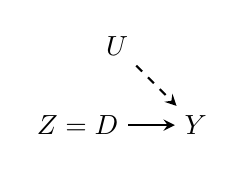
\begin{tikzpicture}
%    \node (z) at (-1,0) {$Z$};
    \node (d) at (0,0) {$Z=D$};
    \node (u) at (0.5, 1) {$U$};
    \node (y) at (1.5,0) {$Y$};
    \draw[->, >=stealth, thick, dashed] (u) -- (y);
 %   \draw[->, >=stealth, thick] (z) -- (d);
    \draw[->, >=stealth, thick] (d) -- (y);
\end{tikzpicture}
\caption{Among compliers}
\end{center}
\column{0.5\textwidth}
\begin{center}
\begin{tikzpicture}
    \node (z) at (-1,0) {$Z$};
    \node (d) at (0,0) {$D$};
    \node (u) at (0.5, 1) {$U$};
    \node (y) at (1.5,0) {$Y$};
    \draw[->, >=stealth, thick, dashed] (u) -- (y);
 %   \draw[->, >=stealth, thick] (z) -- (d);
    \draw[->, >=stealth, thick] (d) -- (y);
\end{tikzpicture}
\caption{Among noncompliers}
\end{center}
\end{columns}
\end{figure}
\end{frame}


\begin{frame}{IV identification in DAGs}
%\vspace{-.2in}
%\begin{figure}
% \begin{columns}
%    \column{0.5\textwidth}
%    \begin{center}
%    \begin{tikzpicture}
%%    \node (z) at (-1,0) {$Z$};
%    \node (d) at (0,0) {$Z=D$};
%    \node (u) at (0.5, 1) {$U$};
%    \node (y) at (1.5,0) {$Y$};
%    \draw[->, >=stealth, thick, dashed] (u) -- (y);
% %   \draw[->, >=stealth, thick] (z) -- (d);
%    \draw[->, >=stealth, thick] (d) -- (y);
%\end{tikzpicture}
%\caption{Among compliers}
%\end{center}
%\column{0.5\textwidth}
%\begin{center}
%\begin{tikzpicture}
%    \node (z) at (-1,0) {$Z$};
%    \node (d) at (0,0) {$D$};
%    \node (u) at (0.5, 1) {$U$};
%    \node (y) at (1.5,0) {$Y$};
%    \draw[->, >=stealth, thick, dashed] (u) -- (y);
% %   \draw[->, >=stealth, thick] (z) -- (d);
%    \draw[->, >=stealth, thick] (d) -- (y);
%\end{tikzpicture}
%\caption{Among noncompliers}
%\end{center}
%\end{columns}
%\end{figure}
\small
\onslide<2-> Further, \\
\small
\begin{itemize}
\item Because $D=Z$ for compliers,  $p(y|do(z))=p(y|do(d))$ for compliers.
\item In full-pop DAG, since $p(d|do(z))$ identified, we can get $p(complier)$.
\end{itemize}

\onslide<3->  Then,
\footnotesize
\begin{align*}
p(y|do(z)) &=  p(y|do(z), \text{comp=1})p(\text{comp=1}) + p(y|do(z), \text{comp=0})p(\text{comp=0}) \\
&= p(y|do(d), \text{comp=1})p(\text{comp=1})  +  p(y| do(d), \text{comp=0})p(\text{comp=0})
\end{align*}

\small
\onslide<4-> Thus for $ ITT= p(y|do(z=1))-p(y|do(z=0)) $ we have
\footnotesize
\begin{align*}
&= [p(y|do(d=1), \text{comp=1})p(\text{comp})  +  p(y| do(d=1), \text{comp=0})p(\text{comp=0})] - \\
& \;\; [p(y|do(d=0), \text{comp=1})p(\text{comp})  +  p(y| do(d=0), \text{comp=0})p(\text{comp=0})] \\
&= [p(y|do(d=1), \text{comp=1}) - p(y|do(d=0), \text{comp=1})]p(\text{comp})  \\
 &= LATE \cdot p(\text{comp=1}) 
\end{align*}
\end{frame}


\begin{frame}{Summary}
\small
\onslide<1-> DAGs communicate the IV setup well, but 
\footnotesize
\begin{itemize}
\item We needed to add in non-NP assumptions. Here, it is that population is split into those with different $D=f_D(U)$ and those with $D=f_D(Z,U)=Z$. 
\smallskip
\item There is nobody for whom $D=f_D(Z,U) = 1-Z$ (monotonicity)
\smallskip
\item $U$ is the cause of compliance (or not); the partition of units into compliers vs. non-compliers relates to a partition of $U$. 
\smallskip
\item It would be interesting to ponder what else can be handled by such population-splitting tricks.
\end{itemize}

\onslide<2-> Back to the big picture:\\
\begin{itemize}
\item IV was our first strategy outside of do-calculus
\item It is very widely used in empirical practice. 
\item We will talk about sensitivity analysis for IV
\item But first we will look at other non-do-calc-identifiable opportunities, i.e. those that flow from imposing other ``non-NP'' type assumptions.
\end{itemize}
\end{frame}

%% =============================================
%% Sensitivity for IV (added 2026-04-29, lifted from sensitivity256.tex)
%% =============================================

\section{Sensitivity for IV (OVB framework)}

\begin{frame}{OVB with instrumental variables}
\small
We can apply the same OVB machinery to IV. Walks through, applied to the Card (1993) returns-to-education example.
\end{frame}


\begin{frame}{Running example: returns to education (Card 1993)}
\small
\begin{itemize}
\item<1-> Estimating returns to education has long been a challenge.
\item<2-> OLS with $N=3010$, covariates $X = \{$race, experience, regional$\}$ suggests 7.5\% higher earnings per year of education.
\item<3-> Confounding may be severe: ability, motivation, family/social.
\item<4-> Card uses \textit{proximity to college} as instrument.
\end{itemize}
\end{frame}


\begin{frame}{These assumptions may fail!}
\small
The IV estimate can be biased --- worse than OLS --- if \textit{Proximity} is not a valid instrument due to uncontrolled:
\smallskip
\begin{itemize}
\item<2-> ``side-effects'' (e.g.\ high-wage jobs near colleges)
\item<3-> ``common-cause confounders'' (e.g.\ unmeasured SES)
\end{itemize}
\onslide<4->
\smallskip
\vspace{-.1in}
\begin{figure}[!ht]
\centering
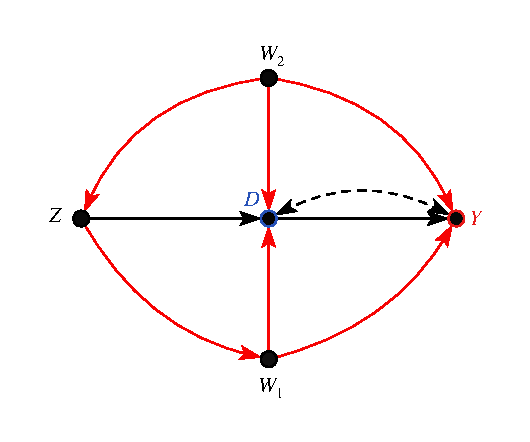
\includegraphics[scale=0.6]{figures/IV_violations_solid.pdf}
\label{fig:bogusIV}
\end{figure}
\vspace{-.3in}
\medskip
\onslide<5->
\begin{center}
\textcolor{blue}{How ``bad'' would such violations need to be to change the conclusion?}
\end{center}
\end{frame}


\begin{frame}{IV regression: three estimators}
\onslide<1-> \textbf{1. Indirect least squares:}
\onslide<2-> \begin{align*}
\text{Reduced form:} & \quad \text{Earnings} = \hat{\lambda}_{\text{res}}\,\text{Proximity} + \X\hat{\beta}_{\text{res}} + \hat{\epsilon}_{y, \text{res}} \\
\text{First stage:} & \quad \text{Education} = \hat{\theta}_{\text{res}}\,\text{Proximity} + \X\hat{\psi}_{\text{res}} + \hat{\epsilon}_{d, \text{res}}
\end{align*}
\bigskip

\onslide<3-> \textbf{2. Two-stage least squares:}
\begin{align*}
\text{2nd stage:} & \quad \text{Earnings} = \hat{\tau}_{\text{2SLS}, \text{res}}\,\widehat{\text{Education}} + \X\hat{\beta}_{\text{2SLS},\text{res}} + \hat{\epsilon}_{\text{2SLS}, \text{res}}
\end{align*}

\onslide<4-> Same answer:
\vspace{-.2in}
\begin{align*}
\hat{\tau}_{\text{2SLS}} = \hat{\tau}_{\text{ILS}} := \frac{\hat{\lambda}_{\text{res}}}{\hat{\theta}_{\text{res}}} = \frac{0.042}{0.319} \approx 0.132.
\end{align*}
\end{frame}


\begin{frame}{IV regression: Anderson--Rubin}
\textbf{3. Anderson--Rubin (Fieller):}
\begin{align*}
\text{Earnings} - \tau_0 \text{Education} = \hat{\phi}_{\tau_0,\text{res}}\,\text{Proximity} + \X\hat{\beta}_{\tau_0,\text{res}} + \hat{\epsilon}_{\tau_0, \text{res}}
\end{align*}
\small
\begin{itemize}
\item $\tau_0$ that makes $\hat{\phi}_{\tau_0,\text{res}} = 0$ is the point estimate
\item $\{\tau_0 : \text{do not reject } \hat{\phi}_{\tau_0,\text{res}} = 0\}$ is the CI
\item Correct coverage regardless of instrument strength
\end{itemize}
\bigskip
\onslide<2-> All give 13.2\% higher earnings per year of education.
\medskip
\begin{center}
\onslide<3-> \textcolor{blue}{How would these change had we included $W$?}
\end{center}
\end{frame}


\begin{frame}{Start with the reduced form}
\onslide<1-> We wanted to run
\begin{align*}
Y = \hat{\lambda}\, Z + \X\hat{\beta} + \hat{\gamma} W + \hat{\epsilon}_y.
\end{align*}
\medskip
\onslide<2-> But $W$ was not observed, so we ran
\begin{align*}
Y = \hat{\lambda}_{\text{res}}\, Z + \X\hat{\beta}_{\text{res}} + \hat{\epsilon}_{y,\text{res}}.
\end{align*}
\medskip
\onslide<3-> \textcolor{blue}{How would including $W$ change inference about $\lambda$?}
\end{frame}


\begin{frame}{Same OVB analysis, different variable names}
\begin{itemize}
\item $R^2_{Y\sim W \mid Z, \X}$: $W$'s share of outcome variance
\item $R^2_{Z\sim W \mid \X}$: $W$'s share of \textit{instrument} variance
\end{itemize}
\onslide<2->
\begin{align*}
|\widehat{\bias}|
&= \sqrt{\frac{R^2_{Y\sim W \mid Z, \X}\, R^2_{Z\sim W \mid \X}}{1 - R^2_{Z\sim W \mid \X}}\,\df}\,\cdot\,\widehat{\se}(\hat{\lambda}_{\text{res}}) \\
&= \BF\sqrt{\df}\,\cdot\,\widehat{\se}(\hat{\lambda}_{\text{res}})
\end{align*}
\onslide<3->
\begin{align*}
\widehat{\se}(\hat{\lambda})
&= \sqrt{\frac{1 - R^2_{Y\sim W \mid Z, \X}}{1 - R^2_{Z\sim W \mid \X}}\,\frac{\df}{\df-1}}\,\cdot\,\widehat{\se}(\hat{\lambda}_{\text{res}}) \\
&= \SeF\sqrt{\df/(\df-1)}\,\cdot\,\widehat{\se}(\hat{\lambda}_{\text{res}})
\end{align*}
\end{frame}


\begin{frame}{An embarrassingly simple sensitivity analysis}
\begin{center}
\textit{Change the critical $t$ rather than the point estimate.}
\end{center}
\medskip

\onslide<2-> Familiar $1-\alpha$ CI:
\begin{align*}
\hat{\lambda}_{\text{res}} \pm t^*_{\alpha, \df} \cdot \widehat{\se}(\hat{\lambda}_{\text{res}}).
\end{align*}

\onslide<3-> Adjust for confounding (limited by $\R^2$):
\begin{align*}
\hat{\lambda}_{\text{res}} \pm \textcolor{blue}{t^\dagger_{\alpha, \df-1, \R^2}} \cdot \widehat{\se}(\hat{\lambda}_{\text{res}}),
\end{align*}

\onslide<4-> where
\begin{align*}
t^\dagger_{\alpha, \df-1, \R^2} := \SeF\sqrt{\df/(\df-1)} \cdot t^*_{\alpha, \df-1} + \BF\sqrt{\df}.
\end{align*}
\end{frame}


\begin{frame}{Routine reporting: (extreme) robustness values}
What would it take to reduce the coefficient until we no longer reject (with confidence $1-\alpha$) that it is $100q\%$ as large?
\bigskip

\onslide<2-> Using the RF coefficient:
\begin{itemize}
\item $\rv_{q,\alpha}(\lambda)$: minimal strength of association with both $Z$ and $Y$ needed.
\medskip
\item $\xrv_{q,\alpha}(\lambda)$: minimal strength with $Z$ alone, even if $W$ explains \textit{all} residual outcome variance.
\end{itemize}
\end{frame}


\begin{frame}{Sensitivity of RF and FS}
\small
\onslide<1-> What can we learn about IV from sensitivity of RF and FS?
\medskip
\onslide<2-> Recall ${\tau} = {\lambda}/{\theta}$.

\onslide<3-> \textbf{Sensitivity of reduced form:} for $H_0: \tau = 0$, sensitivity of RF \textit{is exactly} sensitivity of IV.
\begin{center}
\textit{``If it ain't in the reduced form, it ain't there.''} (Angrist \& Pischke)
\end{center}

\onslide<4-> \textbf{Sensitivity of first stage:} If the sign of the FS isn't guaranteed, you cannot rule out unbounded estimates / CIs.

\onslide<5-> AR is consistent with this logic.
\end{frame}


\begin{frame}{Sensitivity with the AR regression}
\small
\[
Y_{\tau_0} = \hat{\phi}_{\tau_0, \text{res}}\, Z + \X\hat{\beta}_{\tau_0, \text{res}} + \hat{\epsilon}_{\tau_0, \text{res}}
\]

The AR confidence interval:
\begin{align*}
\text{CI}_{1-\alpha}(\tau) = \left\{\tau_0 :\; t^2_{\hat{\phi}_{\text{res}, \tau_0}} \leq (t^*_{\alpha, \df-1})^2\right\}.
\end{align*}

Replace $t^*_{\alpha, \df-1}$ with $t^{\dagger\,\max}_{\alpha, \df-1, \R^2}$:
\begin{align*}
\text{CI}^{\max}_{1-\alpha, \R^2}(\tau) = \left\{\tau_0 :\; t^2_{\hat{\phi}_{\text{res}, \tau_0}} \leq (t^{\dagger\,\max}_{\alpha, \df-1, \R^2})^2\right\}.
\end{align*}
\footnotesize
Analytical solution via quadratic inequality. Yields $\rv_{q,\alpha}(\tau)$, $\xrv_{q,\alpha}(\tau)$ and $\rv_{\geq q,\alpha}(\tau)$, $\xrv_{\geq q,\alpha}(\tau)$.
\end{frame}


\begin{frame}{Card example: sensitivity of RF and FS}
\onslide<2-> \textbf{1. Reduced form: $H: \tau = 0$.}
\footnotesize
\begin{table}[!ht]
\centering
\begin{tabular}{lrrrrrr}
\multicolumn{7}{c}{Outcome: \textit{Earnings} (log)} \\
\hline\hline
Instrument & Est. & SE & t & $R^2_{Y\sim Z \mid \X}$ & $\xrv_{q^*,\alpha}$ & $\rv_{q^*,\alpha}$ \\
\hline
\textit{Proximity} & 0.042 & 0.018 & 2.33 & 0.18\% & 0.05\% & 0.67\% \\
\hline
\multicolumn{7}{l}{\small \textit{Bound (1$\times$ smsa):}\ $R^2_{Y\sim W|Z,\X} = 2\%$,\ $R^2_{Z\sim W|\X} = 0.6\%$,\ $t^\dagger = 2.55$}\\
\multicolumn{7}{l}{\small $\df = 2994,\ q^* = 1,\ \alpha = 0.05$}
\end{tabular}
\end{table}
\normalsize
\bigskip
\onslide<3-> \textbf{2. First stage: stability.}
\footnotesize
\begin{table}[!b]
\centering
\begin{tabular}{lrrrrrr}
\multicolumn{7}{c}{Outcome: \textit{Education} (years)} \\
\hline\hline
Instrument & Est. & SE & t & $R^2_{D\sim Z \mid \X}$ & $\xrv_{q^*,\alpha}$ & $\rv_{q^*,\alpha}$ \\
\hline
\textit{Proximity} & 0.32 & 0.088 & 3.64 & 0.44\% & 0.31\% & 3.02\% \\
\hline
\multicolumn{7}{l}{\small \textit{Bound (1$\times$ smsa):}\ $R^2_{D\sim W|Z,\X} = 0.5\%$,\ $R^2_{Z\sim W|\X} = 0.6\%$,\ $t^\dagger = 2.26$}
\end{tabular}
\end{table}
\end{frame}


\begin{frame}{Card example: reduced form contours}
\begin{figure}[!t]
\centering
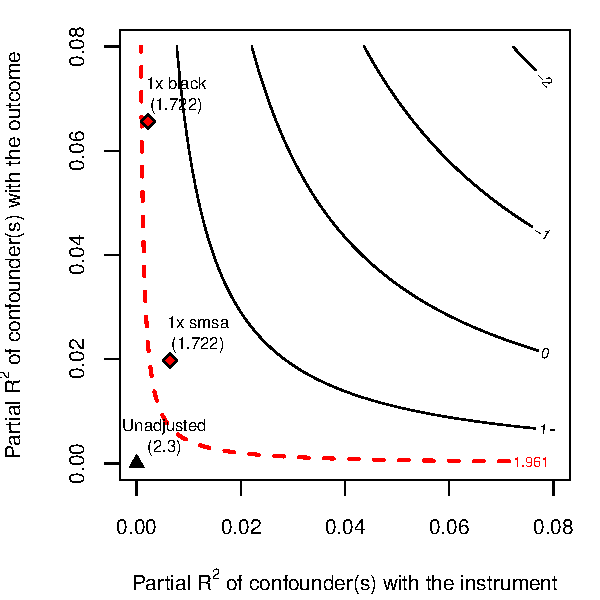
\includegraphics[scale=.75]{figures/card_reduced_form_t-value}
\caption{Sensitivity contours: reduced form}
\end{figure}
\end{frame}


\begin{frame}{Card example: sensitivity of the IV (AR)}
\begin{table}[!ht]
\centering
\begin{tabular}{lrrrrrr}
\multicolumn{7}{c}{Outcome: \textit{Earnings} (log)} \\
\hline\hline
Treatment & Est. & $\text{LL}$ & $\text{UL}$ & t & $\xrv_{\geq q^*,\alpha}$ & $\rv_{\geq q^*,\alpha}$ \\
\hline
\textit{Education} & 0.132 & 0.025 & 0.285 & 2.33 & 0.05\% & 0.67\% \\
\hline
\multicolumn{7}{l}{\small \textit{Bound (1$\times$ smsa):}\ $R^2_{Y_0\sim W|Z,\X} = 2\%$,\ $R^2_{W\sim Z|\X} = 0.6\%$,\ $t^\dagger = 2.55$}\\
\multicolumn{7}{l}{\small $\df = 2994,\ q^* = 1,\ \alpha = 0.05$}
\end{tabular}
\caption{Minimal sensitivity reporting of IV (AR)}
\end{table}

\begin{itemize}
\item<2-> Identical to RF results because the null is $\tau = 0$.
\item<3-> More interesting under other null hypotheses.
\end{itemize}
\end{frame}


\begin{frame}{Card example: CI-limit contours}
\begin{figure}[!b]
\centering
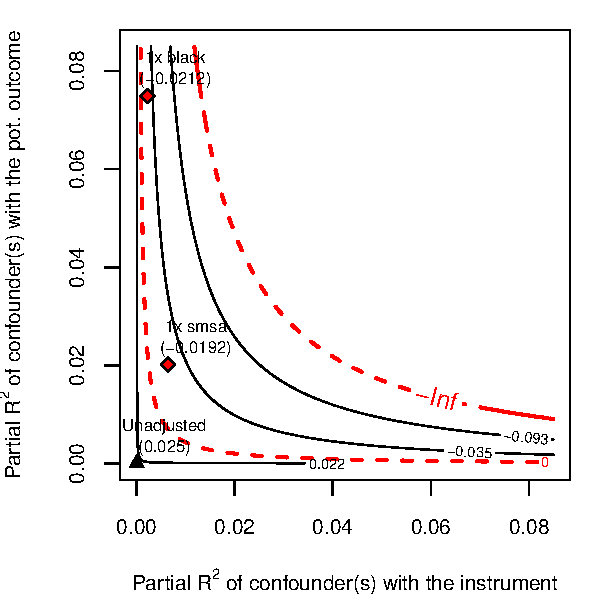
\includegraphics[scale=.6]{figures/card_iv_lower_limit}
\caption{Sensitivity contours: lower 95\% limit}
\end{figure}
\end{frame}


\begin{frame}{IV sensitivity: conclusions}
\begin{itemize}
\item OLS sensitivity to confounding can be as simple as adjusting your critical value.
\item For null of zero in IV, sensitivity of the reduced form \textit{is all you need}.
\item General sensitivity for IV is also easy: in the AR framework, explore how postulated confounding moves point estimates, CI limits, RVs, and bounds.
\end{itemize}
\end{frame}

%% =============================================
%% Appendix begins here
%% =============================================

\appendix

\section{Appendix: SEM / 2SLS framing of IV}

\begin{frame}{IV with constant effects}

\begin{itemize}[<+->]
\item
  Write down a causal model for \(Y_i\) with constant effects and
  an unmeasured confounder, \(U_i\):
  \[Y_i(d,u) = \alpha + \tau d + \gamma u +\eta_i\]
\item Under consistency, 
\[
  Y_i  = \alpha + \tau D_i + \gamma U_i + \eta_i
  \]
\item
 Without $U$, we have error term $\gamma U_i + \eta_i$, and  \(\text{Cov}(\gamma U_i + \eta_i, D_i) \neq 0\).
\end{itemize}

\end{frame}

\begin{frame}{The role of the instrument}
\begin{center}
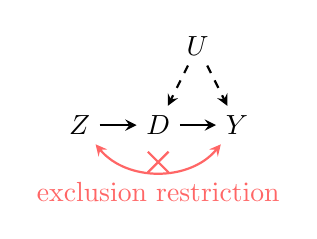
\begin{tikzpicture}
    \node (z1) at (-1,0) {$Z$};
    \node (a1) at (0,0) {$D$};
    \node (l1) at (0.5, 1)
    {$U$};
    \node (y) at
    (1,0) {$Y$};
    \draw[->, >=stealth, thick, dashed] (l1) -- (a1);
    \draw[->, >=stealth, thick, dashed] (l1) --  (y);
    \draw[->, >=stealth, thick] (a1) -- (y);
    \draw[->, >=stealth, thick] (z1) -- (a1);
  \draw[<->, >=stealth, red!60, thick] (z1)  to[bend right = 50] node[cross out, -, draw, red!60, thick, midway] {\vspace{3em}} node[red!60, midway, below] {exclusion restriction}(y);
\end{tikzpicture}
\end{center}

\begin{itemize}[<+->]
\item
  If we have a true instrument \(Z_i\),  then \small \[\text{Cov}(\gamma U_i + \eta_i, Z_i) = 0\]
\item \normalsize Any association of $Y$ and $Z$ is due to $D$. Specifically,
  %It must be independent of \(U_i\) and it has no correlation with
  %\(\eta_i\) because neither does the treatment.
  \pause[\thebeamerpauses]
  \small
  \[\begin{aligned}
  \text{Cov}(Y_i, Z_i) &= \text{Cov}(\alpha + \tau D_i + \gamma U_i + \eta_i, Z_i) \pause \\
  &= \text{Cov}(\alpha, Z_i) + \text{Cov}(\tau D_i, Z_i) + \text{Cov}(\gamma U_i + \eta_i, Z_i) \pause \\
  & = 0 + \tau \text{Cov}(D_i,Z_i) + 0 \\
  & \implies \tau =  \frac{\text{Cov}(Y_i, Z_i)}{\text{Cov}(D_i,Z_i) } 
  \end{aligned}\]
\end{itemize}

\end{frame}

\begin{frame}{IV estimator with constant effects}
\small
\onslide<1-> We can see this as a ratio of two linear regression estimates:
  treatment effect: \[
  \tau = \frac{\text{Cov}(Y_i, Z_i)}{\text{Cov}(D_i, Z_i)} = \frac{\text{Cov}(Y_i, Z_i)/\V[Z_i]}{\text{Cov}(D_i, Z_i)/\V[Z_i]} 
  \] \\
  \medskip
\onslide<2-> So many words and names:
\begin{align*}
Wald = 2SLS = ILS &= \frac{\text{effect of }Z \text{ on } Y} {\text{effect of }Z \text{ on } D} \\
&= \frac{\text{Reduced form effect (aka intent-to-treat)}}{\text{First stage effect}}
\end{align*}
\onslide<3-> With binary instrument, this is merely two DIMs:
  \[
  \tau = \frac{\text{Cov}(Y_i, Z_i)}{\text{Cov}(D_i, Z_i)} = \frac{\E[Y_i|Z_i = 1] - \E[Y_i|Z_i = 0]}{\E[D_i|Z_i = 1] - \E[D_i | Z_i = 0]}
  \]
\onslide<4-> More generically, $$\tau_{IV} = (Z^{\top}X)^{-1}(Z^{\top}Y)$$ where $X$ contains $D$ and any covariates.

\end{frame}

\begin{frame}{Assumptions}
\onslide<1-> Let's take stock of the assumptions we have used: \\
\medskip
\begin{enumerate}
\item Exclusion and exogeneity of instrument
\medskip
\item Relevance
\medskip
\item Constant treatment effects
\end{enumerate}
\end{frame}

\begin{frame}{Weak instruments}
\small
\begin{align*}
 \widehat{\tau}_{IV} &=  \frac{\widehat{\text{Cov}}(Y_i, Z_i)}{\widehat{\text{Cov}}(D_i, Z_i)}\\
 &\inprob \tau + \frac{\text{Cov}(Z_i, U_i)}{\text{Cov}(Z_i,D_i)}
 \end{align*}
 
 \small
\begin{itemize}[<+->]
\item
  If \(\text{Cov}(Z_i, D_i)\) is small, then even very small violations
  of exogeneity \(\text{Cov}(Z_i,U_i) \neq 0\) can lead
  to severe bias.
  \smallskip
\item Can easily be much worse than bias of OLS!
\smallskip
\item  Standard to communicate the strength of the first-stage. $F>10$ is usual rule, but its just a rule.
\smallskip
\item Better: Use Anderson-Rubin approach, which constructs CIs that have correct coverage even with weak instruments
\end{itemize}

\end{frame}

%\begin{frame}
%\begin{center}
%See below for more about this framework and the role of covariates, but for the moment let's stick with the big picture and skip to the ``new'' view of IV.\end{center}
%\end{frame}


\begin{frame}{What about covariates?}

\begin{itemize}[<+->]
\item
  No covariates up until now. What if we have a set of covariates
  \(X_i\) that we are also conditioning on?
\item
  Let's start with linear models for both the outcome and the treatment:
  \[\begin{aligned}
  Y_i &= X_i^{\top}\beta + \tau D_i + \varepsilon_i \\
  D_i &= X_i^{\top}\alpha + \gamma Z_i + \nu_i
  \end{aligned}\]
\item
  Now, we assume that \(X_i\) are \textbf{exogenous} along with \(Z_i\):
  \[Z \perp \nu; \quad Z\perp \varepsilon \]
  \[X \perp \nu; \quad X_i \perp \varepsilon\]
\item
  \ldots{}but \(D_i\) is (still) \textbf{endogenous}:
  \(\E[D_i\varepsilon_i] \neq 0\)
\end{itemize}

\end{frame}

\begin{frame}{Getting the reduced form}

\begin{itemize}[<+->]
\item
  We can plug the treatment equation into the outcome equation:
  \[\begin{aligned}
  Y_i &= X_i^{\top}\beta + \tau[X_i^{\top}\alpha + \gamma Z_i + \nu_i] + \varepsilon_i \pause[\thebeamerpauses]\\
  &= X_i^{\top}\beta + \tau[X_i^{\top}\alpha + \gamma Z_i] + [\tau \nu_i + \varepsilon_i]\pause \\
  &= X_i^{\top}\beta + \tau\alert{[X_i^{\top}\alpha + \gamma Z_i]} + \varepsilon^*_i \pause \\
  &= X_i^{\top}\beta + \tau\alert{\E[D_i|X_i,Z_i]} + \varepsilon^*_i \pause \\
  \end{aligned}\]
\item
  Because \(Z_i\) and \(X_i\) are uncorrelated with \(\nu_i\) and
  \(\varepsilon_i\), then \(\E[D_i|X_i,Z_i]\) is also independent of
  \(\varepsilon^*_i\).
\item
  Thus, the population regression coefficient of a \(Y_i\) on
  \([X^{\top}_i\alpha + \gamma Z_i]\) is the average treatment effect,
  \(\tau\).
\end{itemize}
\end{frame}

%\begin{frame}{Two-stage least squares}
%
%\begin{itemize}[<+->]
%\item
%  Estimate \(\widehat{\alpha}\) and \(\widehat{\gamma}\) from OLS and
%  form fitted values: \[
%  \widehat{\E}[D_i|X_i, Z_i] = \widehat{D}_i = X'_i\widehat{\alpha} + \widehat{\gamma}Z_i.
%  \]
%\item
%  Regress of \(Y_i\) on \(X_i\) and \(\widehat{D}_i\). Add and subtract
%  \(\tau\widehat{D}_i\): \[
%  Y_i = X'_i\beta + \tau \widehat{D}_i + [\varepsilon_i + \tau(D_i - \widehat{D}_i)]
%  \]
%\item
%  Key question: is \(\widehat{D}_i\) uncorrelated with the error?
%\item
%  \(\widehat{D}_i\) is just a function of \(X_i\) and \(Z_i\) so it is
%  uncorrelated with \(\varepsilon_i\).
%\item
%  We also know that \(\widehat{D}_i\) is uncorrelated with
%  \((D_i - \widehat{D}_i)\)?
%\end{itemize}
%
%\end{frame}

\begin{frame}{Two-stage least squares (2SLS)}
 Heuristic procedure:\\
\smallskip
  \begin{enumerate}
  \def\labelenumi{\arabic{enumi}.}
  \item<2->
    Run regression of treatment on covariates and instrument
  \item<3->
    Construct fitted values of treatment
  \item<4->
    Run regression of outcome on covariates and fitted values
  \end{enumerate}
  \begin{itemize}
\item<5->
  This is not how we actually estimate 2SLS because the
  standard errors from second stage are wrong. 
\item<6-> You can instead find that the 2SLS estimator is simply $(\mathbf{Z}^{\top}\mathbf{X})^{-1}(\mathbf{Z}^{\top}Y)$, where $\mathbf{Z}=[X,Z]$,  and $\mathbf{X} = [X, D]$. Can compute SEs from there. 
%
%  Computer wants to calculate the standard errors based on
%  \(\varepsilon^*_i\):
%  \[\varepsilon^*_{i} = Y_i - X'_i\beta - \tau \widehat{D}_i\]
%\item
%  but what we really want is the standard errors based on
%  \(\varepsilon_i\): \[\varepsilon_{i} = Y_i - X'_i\beta - \tau D_i\]
\end{itemize}
\end{frame}

%\begin{frame}{Nunn \& Wantchekon IV example}
%
%\includegraphics{nunn-wantchekon-main.png}
%
%\end{frame}

%\begin{frame}{General 2SLS}
%
%\begin{itemize}[<+->]
%\item
%  Notational convenience: combine \(X_i\) and \(D_i\) into one matrix,
%  \(X_i\), of size \(k\), where one column contains \(D_i\).
%\item
%  The structural model, then is: \[Y_i = X'_i\beta + \varepsilon_i\]
%\item
%  \(Z_i\) will be a vector of \(l\) exogenous variables that includes
%  any exogenous variables in \(X_i\) plus any instruments.
%\item
%  Key assumption on the instruments: \[\E[Z_i\varepsilon_i] = 0\]
%\end{itemize}
%
%\end{frame}
%
%\begin{frame}{Nasty Matrix Algebra}
%
%\begin{itemize}[<+->]
%\item
%  Projection matrix projects values from the columns of \(Z_i\) to the
%  columns of \(X_i\):
%  \[ \Pi = (\E[Z_iZ'_i])^{-1} \E[Z_iX'_i] \qquad \text{(projection matrix)}\]
%  \[ \tilde{X}_i = \Pi'Z_i  \qquad \text{(fitted values)}\]
%\item
%  To derive the 2SLS estimator, take the fitted values, \(\Pi' Z_i\) and
%  multiply both sides of the outcome equation by them:
%  \[ \begin{aligned} Y_i &= X'_i\beta + \varepsilon_i \pause[\thebeamerpauses] \\ \Pi' Z_i Y_i &= \Pi'Z_iX'_i\beta + \Pi' Z_i\varepsilon_i \pause \\  \E[\Pi'Z_i Y_i] &= \E[\Pi'Z_iX'_i]\beta + \E[\Pi'Z_i\varepsilon_i] \pause \\
%  \E[\Pi'Z_i Y_i] &= \E[\Pi'Z_iX'_i]\beta + \Pi'\alert{\E[Z_i\varepsilon_i]} \pause \\
%  \E[\Pi'Z_i Y_i] &= \E[\Pi'Z_iX'_i]\beta \pause \\
%  \E[\tilde{X}_iY_i] &= \E[\tilde{X}_iX'_i]\beta \pause \\
%  \beta &= (\E[\tilde{X}_iX'_i])^{-1}\E[\tilde{X}_iY_i]\end{aligned}\]
%\end{itemize}
%
%\end{frame}
%
%\begin{frame}{How to estimate the parameters}
%
%\begin{itemize}[<+->]
%\item
%  Collect \(X_i\) into a \(n \times k\) matrix
%  \(\X = (X'_1, \ldots, X'_n)\)
%\item
%  Collect \(Z_i\) into a \(n \times l\) matrix
%  \(\mb{Z} = (Z'_1, \ldots, Z'_n)\)
%\item
%  Let \(\widehat{\X} = \mb{Z}(\mb{Z}'\mb{Z})^{-1}\mb{Z}'\X\) be the
%  matrix of fitted values for \(\X\), then we have
%\item
%  Matrix party trick:
%  \(\X'\mb{Z}/n = (1/n)\sum_i^N X_iZ'_i \inprob \E[X_iZ'_i]\).
%\item
%  Take the population formula for the parameters:
%  \[\beta = (\E[\tilde{X}_iX'_i])^{-1}\E[\tilde{X}_iY_i]\]
%\item
%  And plug in the sample values (the \(n\) cancels out):
%  \[\hat{\beta} = (\widehat{\X}'\X)^{-1} \widehat{\X}'\y\]
%\item
%  This is how R/Stata estimates the 2SLS parameters
%\end{itemize}
%
%\end{frame}
%
%\begin{frame}{Asymptotics for 2SLS}
%
%\[\hat{\beta} = (\widehat{\X}'\X)^{-1} \widehat{\X}'\y\]
%
%\begin{itemize}[<+->]
%\item
%  We can insert the true model for \(\y\):
%  \[\hat{\beta} = (\widehat{\X}'\X)^{-1} \widehat{\X}'(\X \beta + \varepsilon)\]
%\item
%  Using the matrix party trick and that
%  \(\widehat{\X}'\X = \widehat{\X}'\widehat{\X}\), we have
%  \[\begin{aligned} \hat{\beta} &= (\widehat{\X}'\X)^{-1} \widehat{\X}'\X\beta + (\widehat{\X}'\X)^{-1} \widehat{\X}'\varepsilon \pause[\thebeamerpauses]\\
%   &= \beta + (\widehat{\X}'\widehat{\X})^{-1} \widehat{\X}'\varepsilon  \pause \\
%   &= \beta + \Big[ n^{-1}\sum_i \widehat{X}_i\widehat{X}'_i \Big]^{-1} n^{-1}\sum_i \widehat{X}_i\varepsilon_i\end{aligned}\]\pause 
%\item
%  Consistent because
%  \(n^{-1} \sum_i \widehat{X}_i\varepsilon_i \inprob \E[\widehat{X}_i\varepsilon_i] = 0\).
%\end{itemize}
%
%\end{frame}
%
%\begin{frame}{Asymptotic variance for 2SLS}
%
%\[\sqrt{n}(\hat{\beta} - \beta) = \Big(n^{-1} \sum_i \widehat{X}_i\widehat{X}'_i\Big)^{-1}\Big(n^{-1/2} \sum_i \widehat{X}_i\varepsilon_i \Big) \]
%
%\begin{itemize}[<+->]
%\item
%  By the CLT, \(n^{-1/2} \sum_i \widehat{X}_i\varepsilon_i\) converges
%  in distribution to \(N(0, B)\), where
%  \(B = \E[\widehat{X}'_i\varepsilon'_i\varepsilon_i\widehat{X}_i]\).
%\item
%  By the LLN,
%  \(n^{-1} \sum_i \widehat{X}_i\widehat{X}'_i \inprob \E[\widehat{X}_i\widehat{X}'_i]\).
%\item
%  Thus, we have that \(\sqrt{n}(\hat{\beta}-\beta)\) has asymptotic
%  variance:
%  \[(\E[\widehat{X}_i\widehat{X}'_i])^{-1}\E[\widehat{X}'_i\varepsilon'_i\varepsilon_i\widehat{X}_i](\E[\widehat{X}_i\widehat{X}'_i])^{-1}\]
%\item
%  Replace with the sample quantities to get estimate of the
%  \textcolor{Blue}{robust 2SLS variance estimator}:
%  \[\widehat{\text{var}}(\hat{\beta}) =  (\widehat{\X}'\widehat{\X})^{-1}\Big(\sum_i \hat{u}^2_i\widehat{X}_i\widehat{X}'_i\Big) (\widehat{\X}'\widehat{\X})^{-1}\]
%  where \(\hat{u}_i = Y_i - X'_i\hat{\beta}\)
%\end{itemize}
%
%\end{frame}

\end{document}
